\section{Usage and Potential Impact Across User Groups}%
\label{sec:usage}

This section explores how the Semantic Web Language Server (SWLS) can be used and the expected impact it has across different user groups.
As a language server, SWLS provides functionality that is independent of specific editors, making it highly versatile.
Some editors, such as NeoVim, treat language servers as first-class citizens, offering seamless integration.
Others, like Visual Studio Code and Monaco, require additional glue code to enable effective interaction.
Regardless of the editor, SWLS delivers a consistent set of features that enhance the user experience across all supported platforms.

All code is under a MIT licence available on github\footnote{\url{https://github.com/ajuvercr/semantic-web-lsp}}.
There are currently three ways to interact with SWLS:
\begin{enumerate}
  \item Download the VSCode extension from the market place\footnote{\url{https://marketplace.visualstudio.com/items?itemName=ajuvercr.semantic-web-lsp}}.
  \item Download and compile the binary locally and integrate it into NeoVim\footnote{Installation instruction are available in the README \url{https://github.com/ajuvercr/semantic-web-lsp}}.
  \item Go to the only demo available on \url{https://swls.ajuvercr.be}.
\end{enumerate}

\todo{Maybe add a screenshot of the editors}
In the demo, users are presented with four distinct editors, each tailored to a specific use case.
A toy ontology and its accompanying SHACL shapes serve as foundational resources for the other editors.
One editor is designed for creating small sample data based on the toy ontology, allowing users to explore how semantic concepts can be applied in practice.
Another editor showcases a simple SPARQL query, which, when executed, provides insights derived from data structured according to the ontology.
This setup allows users to immerse themselves in different personas, gaining hands-on experience with various aspects of semantic data workflows.

While all editors, except for the SPARQL editor, are functionally the same, 
the visual seperation improves the realism of the tasks at hand.
Below, we discuss how SWLS benefits each user group and validate its utility in practice.

We first go over the key ways the SWLS might help users, then we will apply these ways to the different user groups defined in Section \ref{sec:introduction}, 
and how those users groups are theorectially assisted by the SWLS.

\subsection{Key Improvements by SWLS}

The SWLS significantly enhances development efficiency by incorporating robust autocompletion features, shown in Figure \ref{class_completion} and Figure \ref{property_completion}.
These features streamline the creation of semantic documents, enabling users to work faster and with fewer errors. 
Whether defining ontologies, creating SHACL shapes, or writing SPARQL queries, the ability to suggest appropriate classes and properties reduces repetitive tasks and minimizes the cognitive load on users, allowing them to focus on the substance of their work.
Autocompletions also helps user explore the current domain by providing context-aware suggestions.

SWLS also aims to improve comprehension by offering real-time feedback on semantic data.
The hover feature (shown in Figure \ref{hover}), which displays detailed information such as associated classes, allows users to quickly grasp the structure and relationships within a document. 
This instant access to contextual information reduces the need for external references and improves overall productivity.

Finally, SWLS aims to increase user confidence in both syntax and semantics
Syntax validation ensures that documents adhere to the expected standards, catching common mistakes as they occur. This feature is shown in Figure \ref{undefined_prefix}.
For semantic validation, the server highlights SHACL violations, helping users align their documents with structural and logical constraints, shown in Figure \ref{shacl_validation}. 
These validation features not only enhance document quality but also provide educational feedback, aiding users in their journey to master semantic web technologies.

\begin{figure}[h!tb]
    \centering
    % code1
    \begin{subfigure}{0.48\textwidth}
      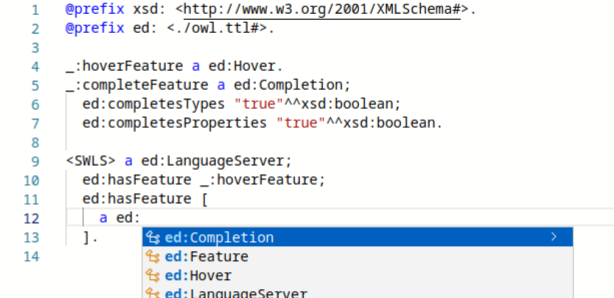
\includegraphics[width=\textwidth]{./images/class_complete.png}
      \caption{SWLS completes a class when the user want to specify the class}
      \label{class_completion}
    \end{subfigure}
    \hfill
    % code 2
    \begin{subfigure}{0.48\textwidth}
      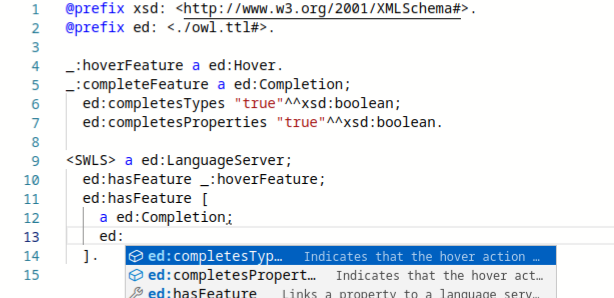
\includegraphics[width=\textwidth]{./images/property_complete.png}
      \caption{SWLS completes properties, first the properties with the correct domain}
      \label{property_completion}
    \end{subfigure}
    \hfill
    % undefined prefix
    \todo{Actually add those screenshots}
    \begin{subfigure}{0.48\textwidth}
      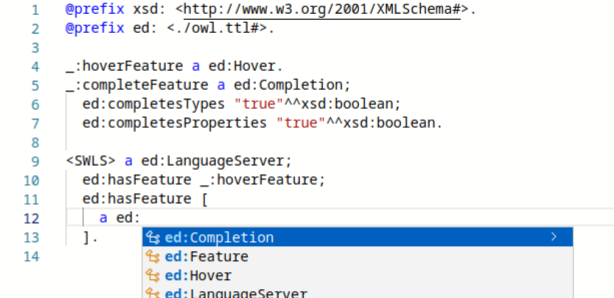
\includegraphics[width=\textwidth]{./images/class_complete.png}
      \caption{SWLS notifies the user of undefined prefixes}
      \label{undefined_prefix}
    \end{subfigure}
    \hfill
    % shacl validation
    \begin{subfigure}{0.48\textwidth}
      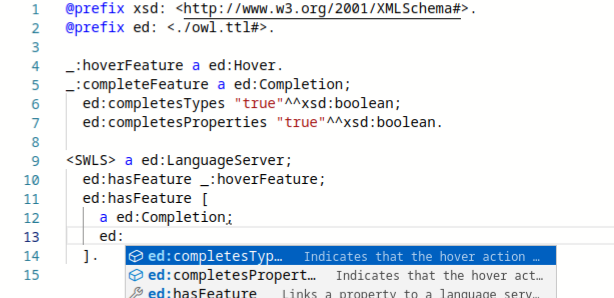
\includegraphics[width=\textwidth]{./images/property_complete.png}
      \caption{SWLS notifies the user of SHACL violations}
      \label{shacl_validation}
    \end{subfigure}
    \hfill
    % shacl validation
    \begin{subfigure}{0.48\textwidth}
      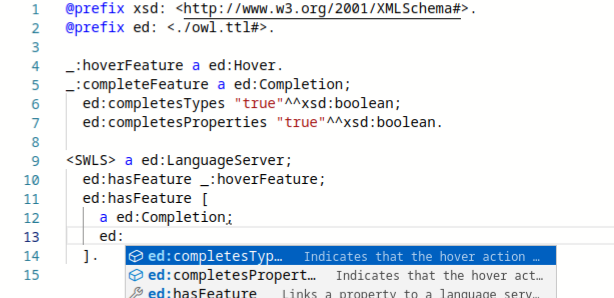
\includegraphics[width=\textwidth]{./images/property_complete.png}
      \caption{SWLS notifies the user of SHACL violations}
      \label{hover}
    \end{subfigure}
    \hfill
    \caption{
      Demo application that shows the usage of SWLS.
      It helps the user by providing autocompletion on classes and properties, taking into account the domain of the properties.
      SWLS also notifies the user of issues like undefined prefixes and SHACL violations.
    }\label{lst:Demo}
\end{figure}

\todo{Add screenshots}

\subsection{User groups}

\paragraph{Semantic power users,} who frequently interact with semantic web technologies, rely on their deep understanding of common properties and domain-specific knowledge to navigate tasks efficiently.
SWLS enhances their workflows by providing robust autocompletion features that streamline document creation and reduce repetitive tasks.
For these users, SWLS also offers a valuable tool for exploring new domains through property suggestions, enabling them to adapt to unfamiliar contexts more easily. 
Additionally, the language server supports quality assurance by helping power users identify common pitfalls such as punning or poorly structured ontologies, ensuring their semantic documents are both accurate and high quality.

\paragraph{For newcomers to the semantic web,} engaging with these technologies can be daunting due to challenges with syntax, semantics, and validation. 
SWLS addresses these pain points by providing immediate feedback on syntax errors, which helps users learn the correct structure and prevents frustration.
The autocompletion feature offers guided support by suggesting relevant properties, allowing users to build confidence in creating semantic documents.
Moreover, validation tools play an educational role: newcomers can intentionally trigger SHACL validation errors to understand what constitutes a faulty document,
turning mistakes into valuable learning opportunities.

\paragraph{Domain experts,} a subset of power users, focus on their specialized fields of knowledge. 
While they share many of the same benefits as general power users, they primarily use SWLS to refine ontologies and ensure alignment with domain-specific standards. 
The autocompletion and hover documentation features help domain experts ensure precision and consistency, facilitating the creation of detailed and accurate semantic models tailored to their expertise.

\paragraph{Data engineers,} on the other hand, primarily work with SPARQL queries to extract meaningful insights from semantic data. 
For these users, SWLS provides critical support by offering autocompletion for classes and properties, as well as syntax validation to prevent errors during query formulation. 
These features significantly enhance productivity by reducing the time spent debugging queries and ensuring accurate results. 
By streamlining the querying process, SWLS enables data engineers to focus on deriving insights rather than resolving technical challenges.


